\section*{Resultados}

La comparación de las segmentaciones obtenidas con el algoritmo y de el histograma se muestra en las siguentes figuras:

\begin{figure}[H]
    \centering
    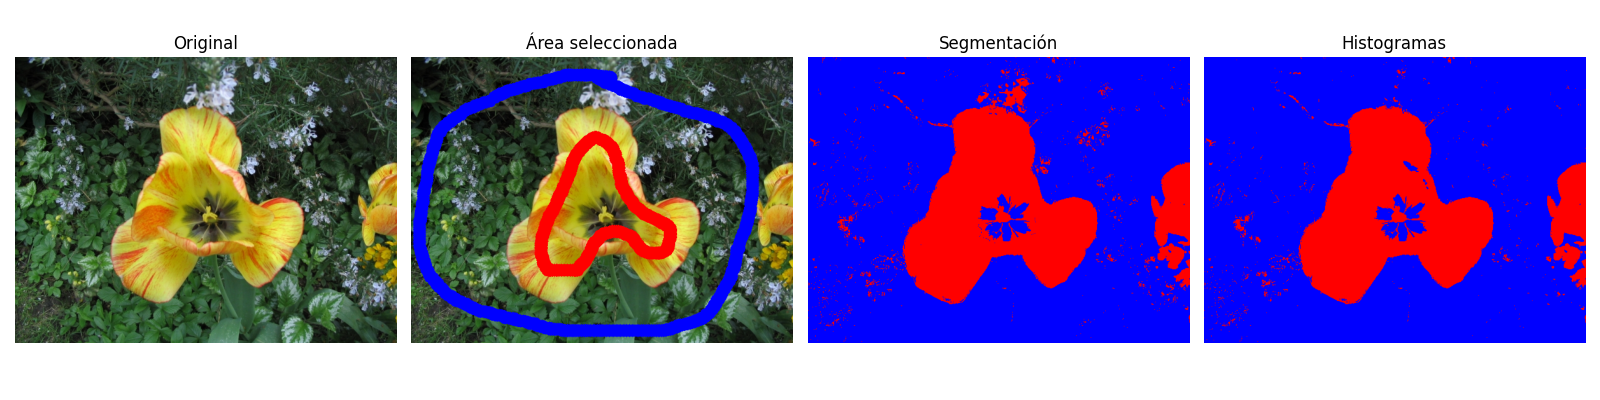
\includegraphics[width=1\linewidth]{Graphics/flower/result.png}
    \caption{Resultados para el archivo \file{flower.bmp}.}
\end{figure}

\begin{figure}[H]
    \centering
    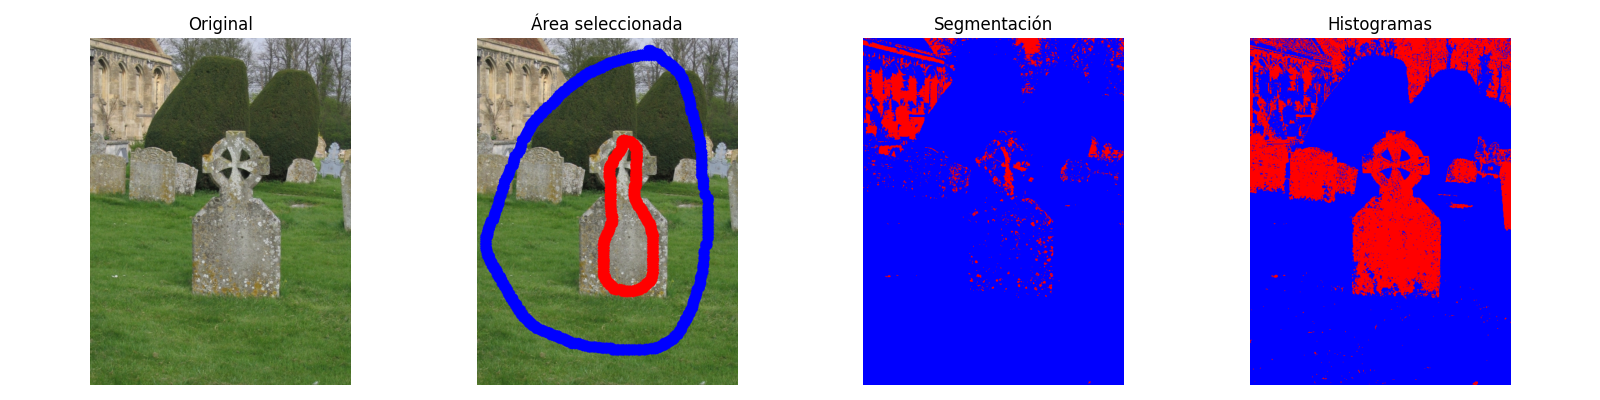
\includegraphics[width=1\linewidth]{Graphics/grave/result.png}
    \caption{Resultados para el archivo \file{grave.bmp}.}
\end{figure}

\begin{figure}[H]
    \centering
    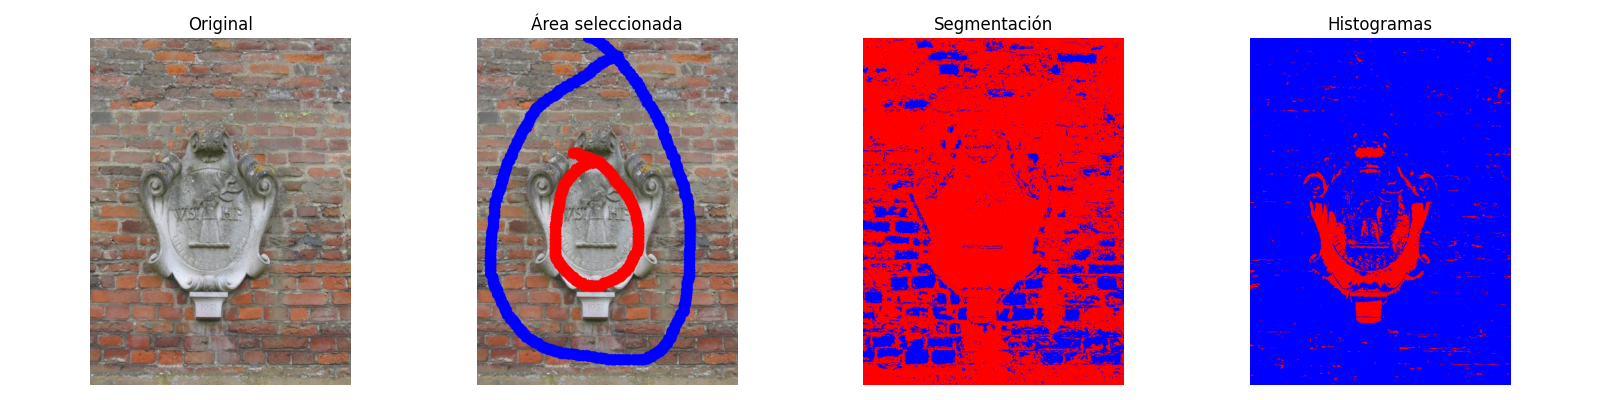
\includegraphics[width=1\linewidth]{Graphics/memorial/result.png}
    \caption{Resultados para el archivo \file{memorial.bmp}.}
\end{figure}

\begin{figure}[H]
    \centering
    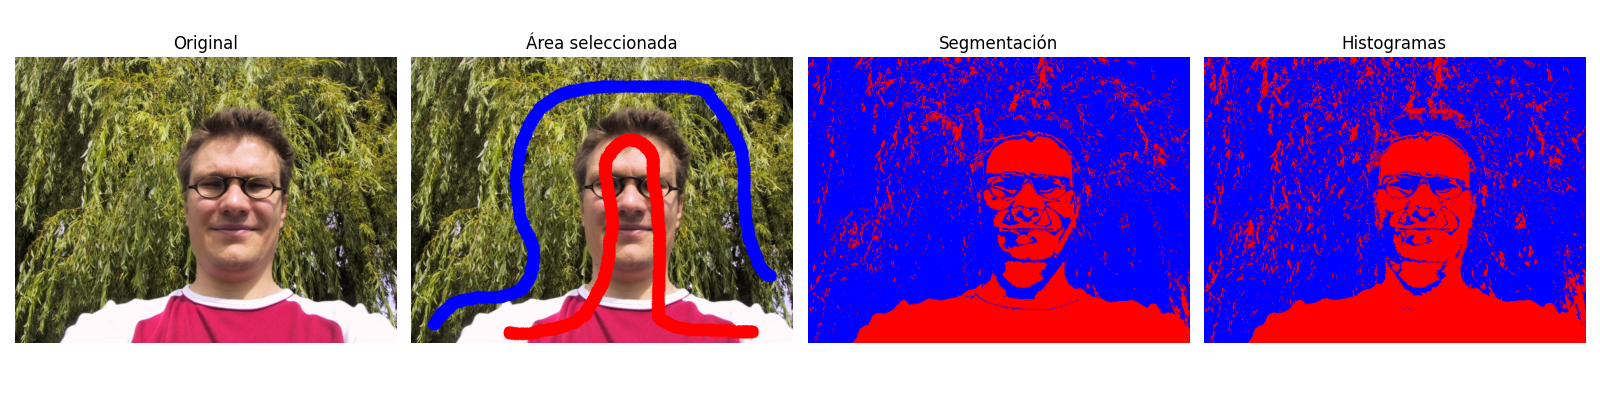
\includegraphics[width=1\linewidth]{Graphics/person1/result.png}
    \caption{Resultados para el archivo \file{person1.bmp}.}
\end{figure}

\begin{figure}[H]
    \centering
    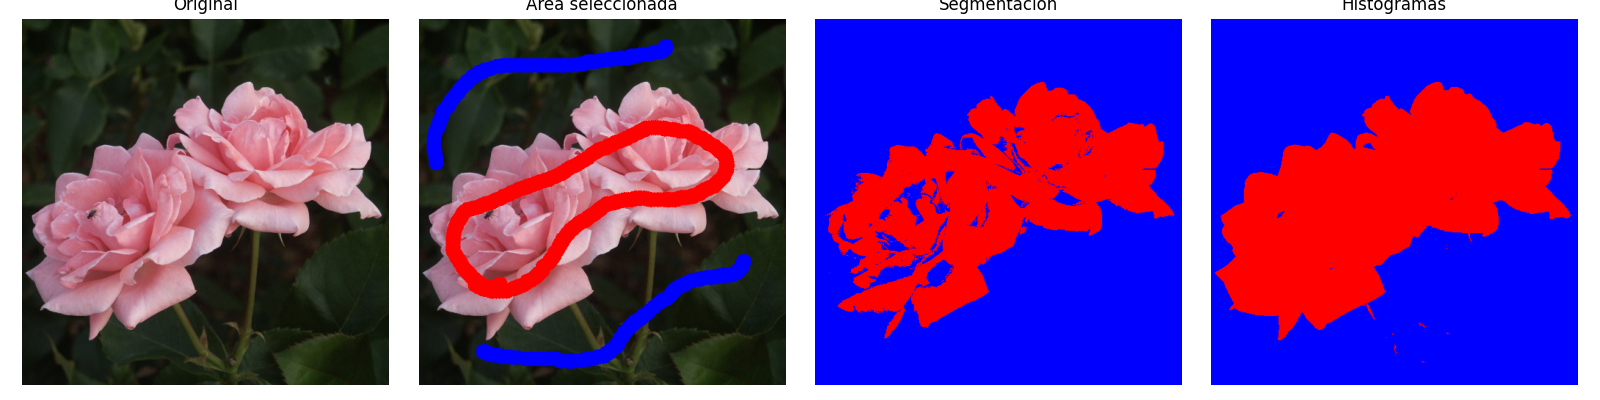
\includegraphics[width=1\linewidth]{Graphics/rose/result.png}
    \caption{Resultados para el archivo \file{rose.bmp}.}
\end{figure}

\begin{figure}[H]
    \centering
    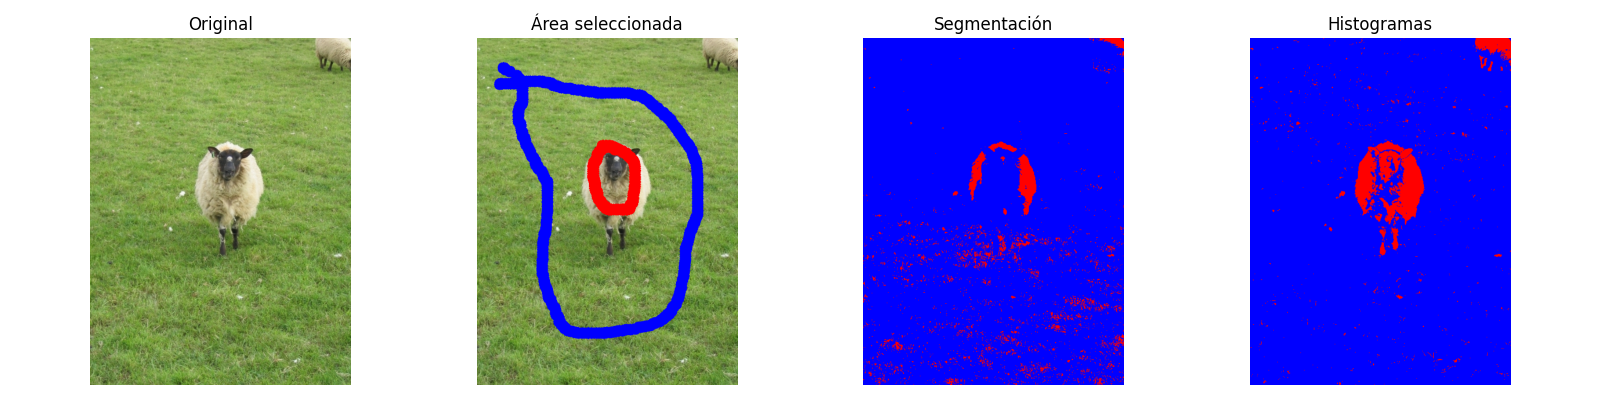
\includegraphics[width=1\linewidth]{Graphics/sheep/result.png}
    \caption{Resultados para el archivo \file{sheep.bmp}.}
\end{figure}

\section*{Conclusiones}

Se observa que el algortimo implementado obtiene resultados semejantes a los histogramas cuando las áreas a segmentar son muy distintas en los colores. Sin embargo en imágenes con tonos y aspectos semejantes, el algoritmo implementado no realiza una buena segmentación de los objetos.